\subsection{Radiação quântica}\label{sec:5.1}
Até agora apenas foi considerada a perda total de energia por radiação síncrotron -- assumindo implicitamente que esta perda de energia é um processo contínuo. Esta análise é satisfatória para uma primeira aproximação já que, na média, a perda de energia é, de fato, suave. Mas já se sabe que toda radiação eletromagnética ocorre em quantidades de energia discreta. E esta discretização da perda de energia impacta significantemente o comportamento dos elétrons no anel de armazenamento.

Cada vez que uma emissão quântica ocorre, a energia do elétron faz um pulo descontínuo. Como será visto depois, as quantidades mais significantes possuem energia em uma faixa desde a luz visível até raio-X mole. Embora tentar explicar quantitativamente os efeitos quânticos pela teoria clássica seja um terreno movediço, as afirmações quase clássicas a seguir podem ser rigorosamente justificadas. Primeiro, o "tempo" durante uma emissão quântica típica não é maior que $\rho/\gamma c$, onde $\rho$ é o raio de curvatura da trajetória e $\gamma$ a energia do elétron em termos da sua energia de repouso. Já que este tempo é muito menor que qualquer outro tempo relevante -- tal como o período de uma oscilação betatron ou de uma oscilação síncroton -- pode-se considerar que esta emissão é instantânea. Segundo, o tempo de cada emissão quântica é estatisticamente independente. Como a mudança de energia em qualquer emissão é uma fração muito pequena da energia do elétron, pode-se considerar que sucessivas emissões são processos puramente randômicos (isto é, com distribuição Poisson).

A mudança descontínua de energia advinda da emissão quântica perturba a trajetória do elétron. O efeito cumulativo de várias perturbações introduzem um tipo de "ruído" nos vários modos de oscilação, fazendo com que suas amplitudes aumentem até que, na média, a excitação quântica seja balanceada pelo amortecimento das oscilações. Este processo será detalhado posteriormente tanto para as oscilações betatron quanto para as oscilações de energia.

Talvez seja necessária aqui uma observação sobre o amortecimento. Nas seções anteriores, os efeitos de amortecimento foram relacionados à radiação. Porém, deve-se notar que o amortecimento depende apenas da taxa média de emissão de energia, e não das suas propriedades estatísticas. Então, ao considerar os efeitos quânticos, deve-se tomar o amortecimento já encontrado -- compreendendo que este ocorre devido à taxa média da perda de energia em todas as energia quânticas. Os efeitos da excitação serão causados pelas flutuações da radiação em torno da sua taxa média (Pode-se, claro, tratar ambos os efeitos da média e da flutuação juntos, porém isto apenas traria complicações indesejadas).

Ao considerar os efeitos das flutuações da radiação nas oscilações de um elétron no anel de armazenamento, deve-se saber certas propriedades sobre radiação quantificada. Então agora estas propriedades serão analisadas.

Do ponto de vista clássico, a radiação síncrona é emitida com um espectro de frequência contínuo. Considere a radiação emitida por um elétron em um intervalo finito de tempo $\Delta t$. Suponha que seja examinado o campo de radiação correspondente -- por um atraso de tempo adequado-- à emissão em $\Delta t$ e, para cada direção no espaço, seja feita uma análise de Fourier deste campo de radiação. O espectro de frequência irá, em geral, ser diferente em cada direção. Mas pode-se tomar a média do espectro em todas as direções a fim de definir o espectro de potência radiada $\mathscr{P}(\omega)$ tal que $\mathscr{P}(\omega)d\omega \Delta t$ seja a energia radiada em $\Delta t$ com frequências angulares entre $\omega e \omega+d\omega$. Claramente, a definição só faz sentido se $\Delta t$ é suficientemente grande de forma que a maioria da energia seja encontrada em frequências maiores que $1/\Delta t$. Relembre que a radiação é tipicamente emitida com um ângulo $1/\gamma$ do vetor de velocidade do elétron. Tal ângulo é varrido para fora no tempo $\rho/\gamma c$, onde $\rho$ é o raio de curvatura local da trajetória. Então um intervalo de tempo $\approx \rho/\gamma c$ deve contar a maioria do impulso de radiação; e, portanto, deve representar uma magnitude adequada para $\Delta t$. Posteriormente será visto que esta ordem de magnitude, de fato, é apropriada.

Com a definição de $\mathscr{P}(\omega)$ dada anteriormente, pode-se permitir que esta seja uma função que varia lentamente com o tempo e, por este fato, não é difícil afirmar que $\mathscr{P}(\omega)$ (e, portanto, suas variáveis de dependência $\rho$ ou $\gamma$) não variam de forma significante em $\Delta t$. Esta condição geralmente é satisfeita\footnote{Os resultados importantes desta parte requerem, na verdade, apenas que $\rho$ e $\gamma$ não mudem significantemente em um tempo $\rho/\gamma^3$, o qual é muito menor que $\Delta t$.} em anéis de armazenamento, então pode-se considerar que $\mathscr{P}(\omega)$ é o espectro de potência "instantâneo" o qual sua integral em $\omega$ é a potência radiada instantânea definida anteriormente,
\begin{align}
	P_\gamma = \int\limits_{0}^{\infty}\mathscr{P}(\omega)\ d\omega
\end{align}

O espectro de potência pode ser escrito num formato mais conveniente:
\begin{align}
	\mathscr{P}(\omega) = \frac{P_\gamma}{\omega_c} S\left(\frac{\omega}{\omega_c}\right)\label{eq:5.2}
\end{align}
com $\omega_c$ a constante definida por
\begin{align}
	\omega_c = \frac{3}{2}\frac{c\gamma^3}{|\rho|}
\end{align}
O número $\omega_c$ é chamado de frequência crítica\footnote{Cuidado! Alguns autores definem a frequência crítica com um fator numérico diferente.}, e note que é aproximadamente igual a $\gamma^3$ vezes a frequência angular de revolução do elétron. A função espectral $S(\omega/\omega_c)$ é uma função puramente algébrica, podendo ser expressada por
\begin{align}
	S(\xi) = \frac{9\sqrt{3}}{8\pi}\xi\int\limits_{\xi}^{\infty}K_{5/3}(\bar{\xi})d\bar{\xi}
\end{align}
onde $K_{5/3}$ é a função de Bessel modificada. Da definição da equação \eqref{eq:5.2}, segue que $S$ é normalizada, então
\begin{align}
	\int\limits_{0}^{\infty}S(\xi)d\xi = 1
\end{align}

\begin{proof}
	Pela definição dada na equação \eqref{eq:5.2}, tem-se que
	\begin{align*}
		P_\gamma = \int\limits_{0}^{\infty}\frac{P_\gamma}{\omega_c} S\left(\frac{\omega}{\omega_c}\right)\ d\omega\\
		\therefore \int\limits_{0}^{\infty}\frac{1}{\omega_c} S\left(\frac{\omega}{\omega_c}\right)\ d\omega = 1
	\end{align*}
	Fazendo uma mudança de variável $\xi = \omega/\omega_c $, tem-se que $d\xi = d\omega/\omega_c$. Logo,
	\begin{align*}
		\int\limits_{0}^{\infty}S(\xi)d\xi = 1
	\end{align*}
\end{proof}

A forma da função de espectro é mostrada na \autoref{fig:fig42}. Seu comportamento para grandes e pequenos argumentos -- o qual pode ser facilmente obtido a partir do comportamento assintótico da função de Bessel -- é útil, às vezes.
\begin{align}
	Para\ \xi<<1;&\ \ \ \ \ S(\xi)\approx 1.34 \xi^{1/3}\nonumber\\
	Para\ \xi>>1;&\ \ \ \ \ S(\xi)\approx \frac{9\sqrt{3}}{8\sqrt{2\pi}} \xi^{1/2}e^{-\xi}\label{eq:5.6}
\end{align}

\begin{figure}[!htb]
	\centering
	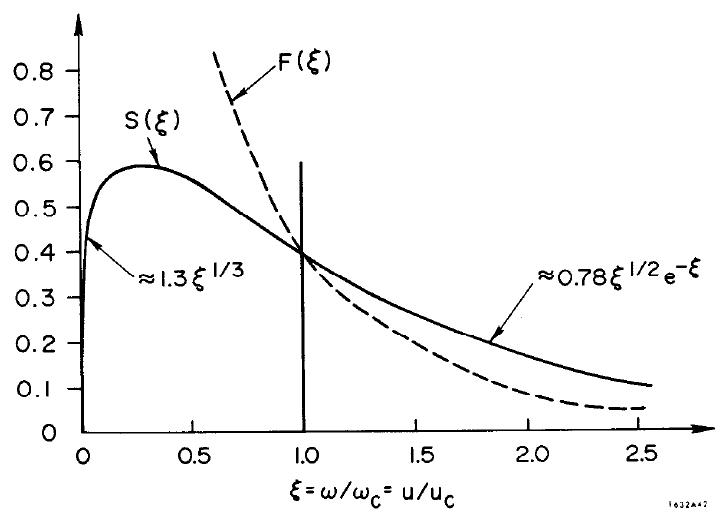
\includegraphics[width=0.7\linewidth]{./Figuras/fig42.jpeg}
	\caption{Espectro de potência normalizado $S$ e espectro do número de fótons $F$ da radiação síncrona. Retirado de \cite{sands1970physics}.}
	\label{fig:fig42}
\end{figure}

O espectro de potência $\mathscr{P}(\omega)$ é obtido a partir de $S(\xi)$ pela equação \eqref{eq:5.2}. Não esqueça que tanto $P_\gamma$ -- veja a equação \eqref{eq:4.4} -- quanto $\omega_c$ dependem de $\gamma$ e $\rho$. Fica claro a partir da \autoref{fig:fig42} que a maioria da potência é encontrada em frequências próximas de $\omega_c$ (como $\omega_c$ é $\gamma^2$ vezes maior que o inverso de $\Delta t$ definido antes, as suposições feitas estão justificadas).

É sabido que a radiação eletromagnética na frequência angular $\omega$ é emitida em uma quantidade de energia $u=\hslash \omega$, onde $\hslash$ é a constante de Plank reduzida por $2\pi$ ($\hslash = h/2\pi = 6.85 \times 10^{-16} eVs$). Seja $n(u)du$ o número de quantidade de energia emitida por unidade de tempo com energias entre $u$ e $u+du$. A potência emitida nessa quantidade é $u n(u)du$, a qual deve ser igual a potência emitida no intervalo de frequência $d\omega = du/\hslash$ na frequência $\omega = u/\hslash$, ou seja,
\begin{align}
	un(u)du = \mathscr{P}(u/\hslash)du/\hslash
\end{align}
Tomando $\mathscr{P}(\omega)$ da equação \eqref{eq:5.2}, a função da distribuição quântica pode ser escrita como
\begin{align}
	n(u) = \frac{P_\gamma}{u_c^2}F\left(\frac{u}{u_c}\right)
\end{align}
com
\begin{align}
	u_c = \hslash \omega_c = \frac{3}{2}\frac{\hslash c \gamma^3}{|\rho|}\label{eq:5.9}\\
	F(\xi) = \frac{1}{\xi}S(\xi)
\end{align}
Como o espectro de frequência, o espectro quântico é, a menos de um fator de escala $P_\gamma/u_c^2$, uma função universal de relação $u/u_c$.

A função $F(\xi)$ também é representada na \autoref{fig:fig42}. A taxa de emissão quântica por unidade de intervalo de energia diverge em pequenas energias\footnote{O espectro é, de qualquer forma, questionável para $u<u_c/\gamma^3$, de acordo com as condições mencionadas anteriormente}. Mas apenas como $u^{-2/3}$, então a taxa de emissão em qualquer intervalo finito de energias quânticas -- uma integral em $u$ -- é finita.

Seja $\mathscr{N}$ a taxa total de emissão quântica (para todas as energias):
\begin{align}
	\mathscr{N} = \int\limits_{0}^{\infty}n(u)du
\end{align}
A partir das expressões assintóticas para $S(\xi)$ na equação \eqref{eq:5.6}, uma integral completa é aproximadamente 1. Na verdade, seu valor exato é $15\sqrt{3}/8$, então
\begin{align}
	\mathscr{N} = \frac{15\sqrt{3}}{8}\frac{P_\gamma}{u_c}\label{eq:5.12}
\end{align}
A energia quântica média é definida como
\begin{align}
	\mean{u} = \frac{1}{\mathscr{N}}\int\limits_{0}^{\infty}un(u)du
\end{align}
A integral é apenas $P_\gamma$, então a energia quântica média é
\begin{align}
	\mean{u} = \frac{8}{15\sqrt{3}}u_c = (0.32...)u_c
\end{align}
Falando grosseiramente, pode-se dizer que a radiação é emitida em quantidades de energia em torno de $u_c$, e com uma taxa média em torno de $P_\gamma/u_c$. Para um elétron com 1GeV movendo-se em uma trajetória com raio de curvatura de 5m,
\begin{align*}
	P_\gamma =& 1.7 \times 10^11\ eVs^{-1}\\
	u_c =& 437\ eV\\
	\mathscr{N} =& 3.2 P_\gamma/u_c = 1.3 \times 10^9\ s^{-1}
\end{align*}

É interessante notar que o número médio de quantidade de energia emitida por radiano da trajetória depende apenas da energia do elétron. Isto é, de fato, quase igual a apenas multiplicar $\gamma$ pela constante estrutural:
\begin{align}
	n\acute{u}mero\ m\acute{e}dio\ de\ energia\ qu\hat{a}ntica\ emitida\ por\ radiano = \frac{5}{2\sqrt{3}}\frac{\gamma}{137}
\end{align}
Para um elétron de 1GeV, o número é em torno de 20. O número real em qualquer intervalo de tempo flutua seguindo uma distribuição Poisson correspondente ao número médio. Portanto, em pequenos números, as flutuações são significativas.

Será visto depois que a excitação quântica das oscilações de um elétron em um anel de armazenamento depende não apenas da taxa média de emissão quântica, mas também da média quadrada da energia quântica. Deve-se esperar que $\mean{u^2}$ seja em torno de $u_c^2$; o que, de fato, é. Analisando detalhadamente, pode-se chegar que
\begin{align}
	\mean{u^2} = \frac{11}{22}u_c^2
\end{align}
Uma quantidade que irá entrar na excitação quântica das oscilações é, de fato, o produto entre a média quadrada da energia quântica e a taxa média $\mathscr{N}$; ou seja,
\begin{align}
	\mathscr{N}\mean{u^2} = \int\limits_{0}^{\infty}u^2n(u)du\label{eq:5.17}
\end{align}
Utilizando a equação \eqref{eq:5.12}, será conveniente escrever
\begin{align}
	\mathscr{N}\mean{u^2} = C_u u_c P_\gamma\label{eq:5.18}
\end{align}
com
\begin{align}
	C_u = \frac{55}{24\sqrt{3}} = 1.32...
\end{align}

É importante manter em mente que tanto $u_c$ quanto $P_\gamma$ são funções da energia do elétron e do raio de curvatura local da trajetória. Tomando $u_c$ da equação \eqref{eq:5.9} e $P_\gamma$ da equação \eqref{eq:4.4},
\begin{align}
	\mathscr{N}\mean{u^2} = \frac{3C_u C_\gamma}{4\pi}\frac{\hslash c^2}{(mc^2)^3}\frac{E^7}{\rho^3} = \frac{55}{24\sqrt{3}}r_e \hslash mc^4 \frac{\gamma^7}{|\rho^3|}
\end{align}
Para um raio de curvatura fixo, a excitação quântica varia com a sétima potência da energia!